%算法部分的写作思路:
%	首先该部分为两个大的小节:
%		1、三元祖提取:
%			NLP的角度进行解释分词和三元组提取
%		2、布局优化算法:
%			将如何设立优化目的、如何确定约束条件等
%突出布局的目的是在故事线中更多的展示实体之间的联系
	
\section{Vis Tech}
% 我们介绍一种新的模式挖掘方法来发现实体间的关系和具体实体的作用。在本节我们首先简要介绍了自然语言处理领域中的三元组抽取,以此为输入数据,然后详细演示了我们的算法实现。
\noindent  We introduce a new pattern mining method to discover the relationships between entities and the role of specific entities. In this section we first briefly introduce triple extraction in the field of natural language processing as input data, and then demonstrate our algorithm implementation in detail.

\subsection{Inter-entity relation extraction}
%正如3.1节中提到的,为了突出展示实体间的关系,SPO三元组是非常适合的。本节将简要说明我们如何获得SPO三元组。
\noindent As mentioned in Section 3.1, in order to highlight the relationship between entities, SPO triples are very suitable. This section will briefly explain how we obtain SPO triples.

%在自然语言处理中,依存关系分析的结果是一个有向图G=(V,A)。V代表节点,即句子中的每一个词;A代表有向边,表示词之间的依存关系。其结构通常是数据结构中的树。依存句法分析和语义依存分析都是依存关系分析的方法。前者注重句法结构,后者注重语义关联。我们借助自然语言处理的工具HanLP,对原始数据进行处理。首先,我们使用HanLP中的依存句法分析和语义依存分析,将文本数据转换成依存关系树。对例句"Tom eats oranges today.",其结构如图DT所示。从中我们可以看到,依存句法树标识了语法成分,语义依存标识了语义关系。接着,根据两者的不同特性,我们可以对两者的每个节点进行遍历。从依存句法树中选取满足主谓关系(SBV)和动宾关系(VOB)的节点;从语义依存树中得到相同节点的语义关系,用来判断主被动。最后将得到的节点进行组合,变成SPO三元组。依存句法分析的结果为,SBV:eats->Tom, VOB:eats->oranges;语义依存分析的结果为,Agt:eat->Tom,Pat:eat->oranges。由此可知,该句的SPO三元组为<Tom-eats-oranges>,Tom是施者,oranges是受者。
In natural language processing, the result of dependency analysis is a directed graph \textit{\textbf{G=(V,A)}}. \textit{\textbf{V}} represents a node, that is, each word in the sentence; \textit{\textbf{A}} represents a directed edge, representing the dependency between words. Its structure is usually a tree. Dependency syntax analysis and semantic dependency analysis are both methods of dependency analysis. The former focuses on syntactic structure, while the latter focuses on semantic association. We use the natural language processing tool \textbf{HanLP}~\cite{noauthor_hanlp_nodate} to process the raw data. First, we convert text data into a dependency tree using dependency parsing and semantic dependency parsing in HanLP. For the example,  \textit{"Tom eats oranges today."}, its structure is shown in Fig~\ref{fig:DT}. From this we can see that the dependency syntax tree identifies syntactic components, and the semantic dependency identifies semantic relations. Then, according to the different characteristics, we can traverse each node of the two. Select the nodes that satisfy the subject-verb relationship (SBV) and the verb-object relationship (VOB) from the dependency syntax tree; get the semantic relationship of the same node from the semantic dependency tree, which is used to judge the active and passive. Finally, the obtained nodes are combined into SPO triples. The result of the dependency syntax analysis is, SBV: \textit{Tom$\gets$eats}, VOB: \textit{eats$\to$oranges}; the result of the semantic dependency analysis is, Agt: \textit{Tom$\gets$eats}, Pat: \textit{eat$\to$oranges}. It can be seen that the SPO triple of this sentence is $<$\textit{Tom-eats-oranges}$>$, \textit{Tom} is the giver, and \textit{oranges} is the receiver.
 
\begin{figure}[h]
	\centering
	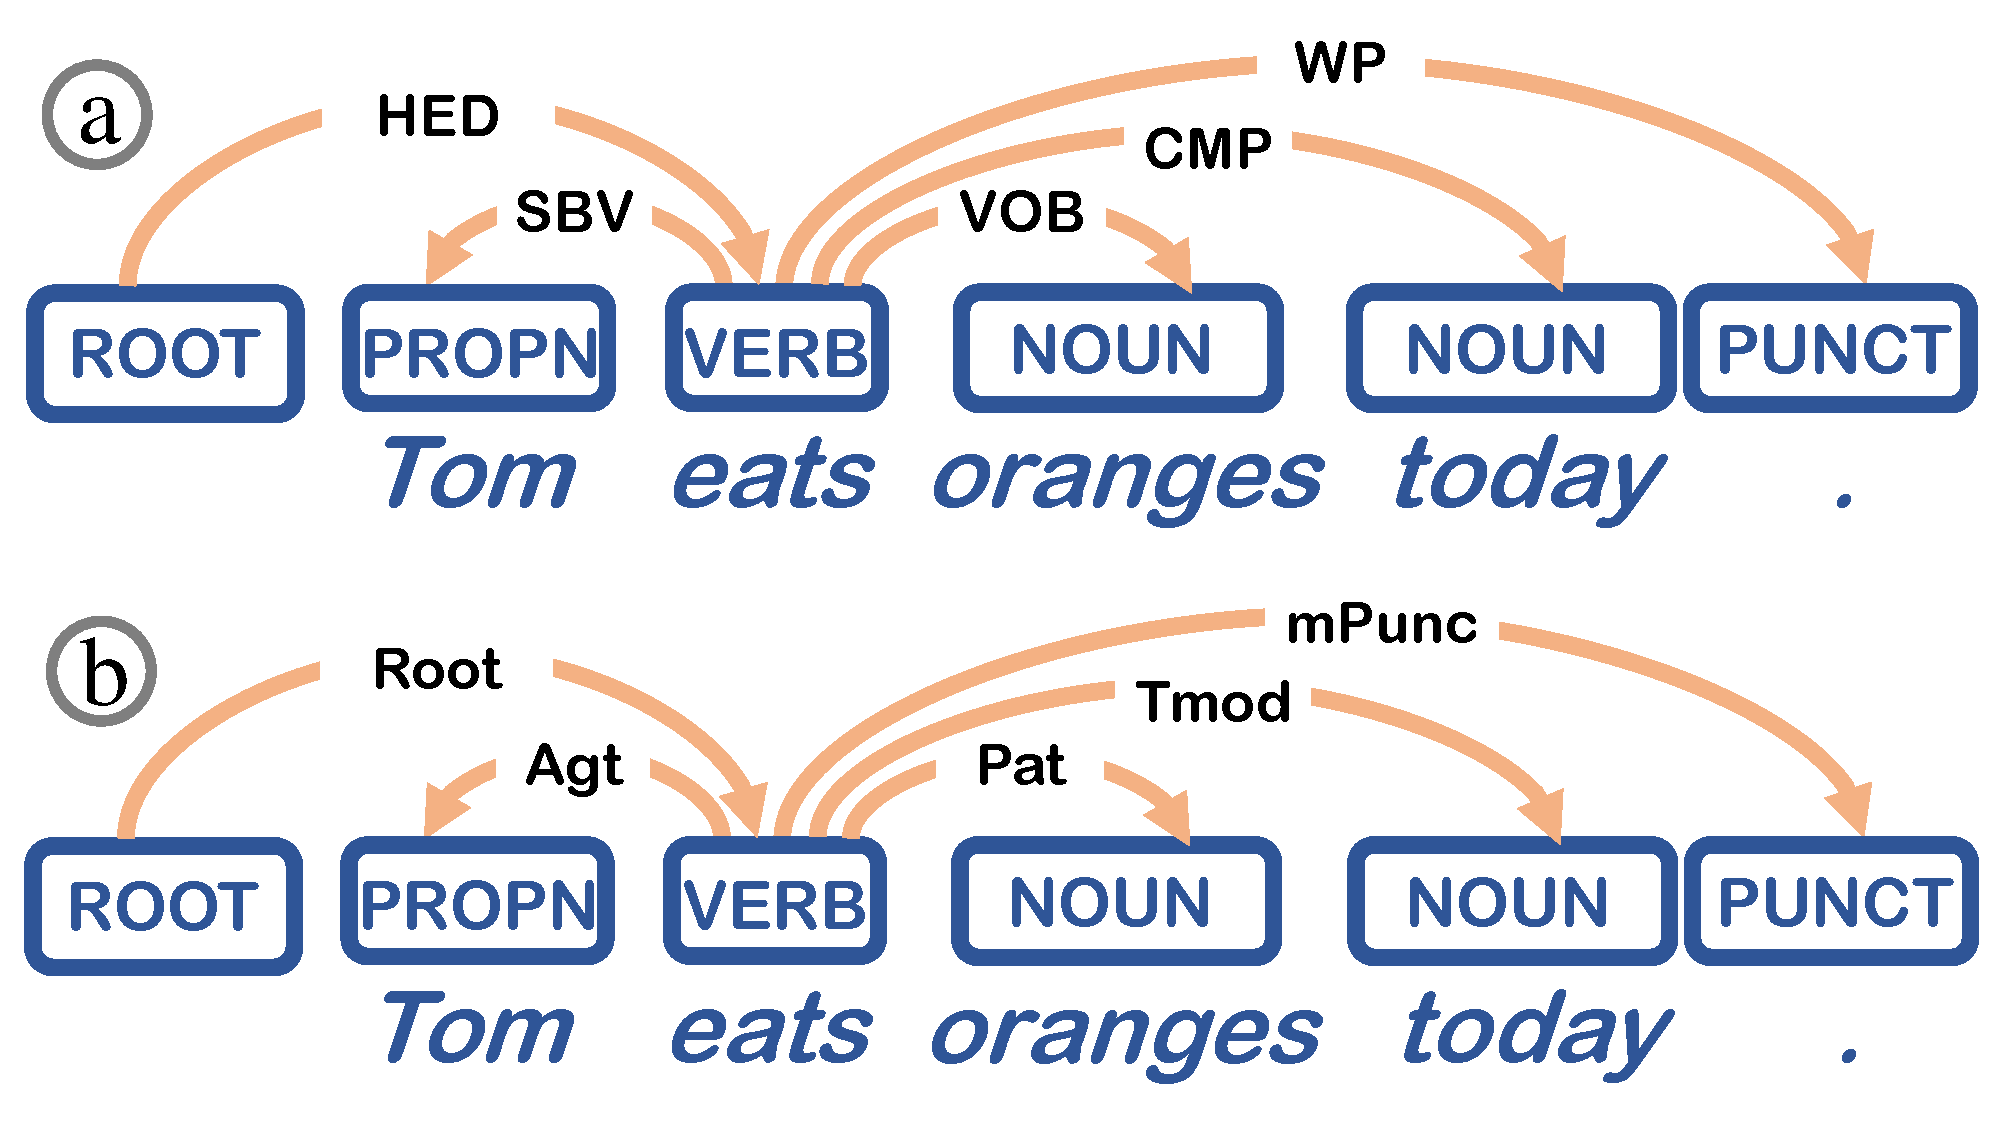
\includegraphics[width=0.48\textwidth]{Fig/dt1.pdf}
	\vspace{-0.5em}
	\caption{dt}
	\vspace{-1.5em}
	\label{fig:DT}
\end{figure} 

%原始数据经过上述流程处理后,就可以获得具有主被动信息的SPO三元组。
After the original data is processed through the above process, the SPO triples with active and passive information can be obtained.

%布局算法实现
\subsection{Layout algorithm implementation}
%遵从3.2小节提出的设计需求,我们将从选取优化目标,数学表达两个部分,详细阐述布局算法的实现。
\noindent  Following the design requirements proposed in Section 3.2, we will discuss the implementation of the layout algorithm in detail from the selection of optimization objective and the mathematical expression.

%选取优化目标
\subsubsection{Selection of optimization objective}
%在传统故事线中添加事件,并展示实体与实体之间关系是个新颖的尝试。现有关于故事线的工作大部分也是关于布局优化。但由于数据类型、展示意图不同,优化算法的侧重点也会大相径庭。
\noindent Adding events to traditional storylines and showing relationships between entities is a novel attempt. Much of the existing work on storylines is also about layout optimization. However, due to the different data types and diagrams, the focus of the optimization algorithm will be quite different. 

%将设计需求转换成数学问题是与提出完善的设计需求同等重要的。例如,HDR1中将每个实体编码成连续的线条,但是实体之间是离散的。因此,在同一时刻的实体位置可以转换成“分配问题”。我们的工作是围绕获得简洁、可读性强的故事线可视化展开的,换而言之就是减少故事线的复杂程度。在列举的设计需求中,SD1、SD2以及CD1,都是为此提出的。虽然SD1和SD2,分别针对的是减少点和线的复杂程度,但归根到底都是减少交点的数量。我们将线交点最少,作为优化目标1;CDR2中同一事件中的同一SPO三元组的实体尽可能靠近,作为优化目标2。综合HDR1、SDR1以及CDR2,我们其描述成多目标优化问题。
Translating design requirements into mathematical problems is as important as formulating sound design requirements. For example, each entity is encoded as a continuous line in HDR1, but the entities are discrete. Therefore, the physical location at the same time can be transformed into an "\textit{Allocation Problem}". Our work revolves around getting a concise, readable visualization of the storyline, in other w ords, reducing the complexity of the storyline. Among the design requirements listed, SDR1, SDR2 and CD1 are all proposed for this purpose. Although SDR1 and SDR2 are aimed at reducing the complexity of points and lines, respectively, they are all about reducing the number of intersections. We take the least number of line intersections as optimization objective 1 \textbf{(op1)}; the entities of the same SPO triplet in the same event in CDR2 are as close as possible to each other as optimization objective 2 \textbf{(op2)}. Combining HDR1, SDR1 and CDR2, we its described as a multi-objective optimization problem.

%4.2.2数学表达
\subsubsection{Mathematical expression}
%选好优化目标,紧接着要做的是将其转换成正确的数学表达。
\noindent Once the optimization objective has been chosen, the next thing to do is to convert it into the correct mathematical expression.

%op1: 可以通过比较相邻时刻实体i和j的纵坐标,来表示两条线之间是否存在交叉。我们定义yit,表示实体i在t时刻的纵坐标。如果实体i和实体j相交,则$(y_{it}-y_{jt})(y_{i,t+1}-y_{j,t+1})<0$。要使交叉点的数量最小化,优化目标1可以将表达为:
$\blacksquare $ \textbf{op1:} The existence of a cross can be indicated by comparing the vertical coordinates of entities $i$ and $j$ at adjacent moments. We define $y_{i,t}$, which denotes the longitudinal coordinate of entity $i$ at moment $t$. If there is an intersection, then $(y_{it}-y_{jt})(y_{i,t+1}-y_{j,t+1})<0$. To minimize the number of intersections, the op1 can be expressed as

%公式1
\begin{equation}
	min \quad  \frac{1}{2}\sum_{i,j}\sum_{t}\mathbb{I}_{\{(y_{i,t}-y_{j,t})(y_{i,t+1}-y_{j,t+1})<0 \}}
\end{equation}

%考虑到上述表达式中较为繁琐,我们引入Pijt和oith。两者都是0-1决策变量。前者用来判断在t时刻,第i个实体是否在第j个实体的下方。如果$y_{i,t}<y_{j,t}$,则Pijt为1,否则为0。后者用来判断实体i在时刻t在队列中的位置。如果实体i的位置为h,则oith为1,否则为0。$o_{i,t,h}$与$y_{i,t}$的数学关系可以表示成:
Considering that the above expressions are more cumbersome, we introduce $o_{i,j,t}$ and $o_{i,t,h}$. both of which are 0-1 decision variables. The former is used to determine whether the entity $i$ is below the entity $j$ at moment $t$. If $y_{i,t}<y_{j,t}$, $p_{i,j,t}$ is 1, otherwise it is 0. The latter is used to determine the position of entity $i$ in the queue at moment $t$. If the position of entity $i$ is $h$, then $o_{i,t,h}$ is 1, otherwise it is 0. The mathematical relationship between $o_{i,t,h}$ and $y_{i,t}$ can be expressed as:

%公式2
\begin{equation}
y_{i,t} =  \sum_{h}o_{i,t,h}h \quad\quad 
\end{equation}


%$O_{i,t,h}$和$P_{i,j,t}$之间的数学关系可以表示为:
\noindent The mathematical relationship between $o_{i,t,h}$ and $p_{i,j,t}$ can be expressed as:

%公式3
\begin{equation}
p_{i,j,t} = 1, \quad\quad when\quad o_{i,t,h1} + o_{j,t,h2}=2\;\&\;h1<h2
\end{equation}

%至此,我们可以将公式(1)简化为:
\noindent At this point, we can simplify Eq.(1) as:

%公式4
\begin{equation}
	min \quad \sum_{i,j,t}p_{i,j,t}p_{j,i,t+1}
\end{equation}

%op2: 对op2,我们可以把它转述为,在同一时刻t,有联系的两个实体i和j之间的纵坐标差值最小。为了指定适用的实体,减少计算量,我们引入两个0-1常量,$C_{i,e}$和$B_{e,t}$。$C_{i,e}$指实体i参与了事件e。$B_{e,t}$指t时刻发生的是事件e。在数学上说,op2可以表达为:
$\blacksquare$ \textbf{op2:} For op2, we can paraphrase it as, at the same moment $t$, the difference in vertical coordinates between two entities $i$ and $j$ that are connected has the smallest value. To specify the applicable entities and reduce the computational effort, we introduce two 0-1 constants, $C_{i,e}$ and $B_{e,t}$. $C_{i,e}$ means that entity $i$ is involved in event $e$. $B_{e,t}$ means that it is event $e$ that occurs at moment $t$. Mathematically speaking, op2 can be expressed as:

%公式5
\begin{equation}
	min \quad \sum_{i,j,t,e,h}(o_{i,t,h}-o_{j,t,h})^2B_{e,t}C_{i,e}C_{j,e}
\end{equation}

%将op1和op2结合,就可以得到完整的多目标优化方程。$\alpha$ 和 $\beta$是多目标优化方程求解时的权重。在经过多次实验后,我们将$\alpha$ 和 $\beta$的值分别设置为1和0.2。
The complete multi-objective optimization equation can be obtained by combining op1 and op2. $\alpha$ and $\beta$ are the weights when solving the multi-objective optimization equation. After several experiments, we set the values of $\alpha$ and $\beta$ to 1 and 0.2, respectively.

%公式6
\begin{equation}
\begin{split}
min \quad \alpha\sum_{i,j,t}p_{i,j,t}p_{j,i,t+1} + 
\beta\sum_{i,j,t,e,h}(o_{i,t,h}-o_{j,t,h})^2B_{e,t}C_{i,e}C_{j,e}
\end{split}
\end{equation}

%首先写的是指派问题
%约束:首先,我们将实体的排序转换为“指派问题”。假设我们有$H$个箱子组成的队列,在t时刻,实体i必须且只能进一个箱子$h$。为了将该问题转换成数学表达式,我们可以使用变量$O_{i,t,h}$和$P_{i,j,t}$,h1和h2分别为实体i和j在t时刻在队列中的位置。“指派问题”可以表达为:
$\blacksquare$ \textbf{Constraints:} First, we transform the ordering of entities into an "\textbf{assignment problem}". Suppose we have a queue of $H$ boxes and at time $t$, entity $i$ must and can enter only one box $h$. To convert this problem into a mathematical expression, we can use the variables $o_{i,t,h}$ and $o_{i,j,t}$, with $h1$ and $h2$ being the positions of entities $i$ and $j$ in the queue, respectively. The "assignment problem" can be expressed as follows:

%公式7
\begin{subequations}
	\begin{align}
		\sum_io_{i,t,h}&=1, \quad\quad \forall t,h \\
		\sum_ho_{i,t,h}&=1, \quad\quad \forall i,t \\
		p_{i,j,t}+p_{j,i,t}&=1, \quad\quad \forall t,i,j\;\&\;i \neq j\\
		p_{i,j,t}&=0, \quad\quad \forall t,i=j 
	\end{align}
\end{subequations}

%公式(7a)确保对每个实体$i$,在任意的t时刻,只可以在队列中占据一个位置。公式(7b)确保在任意的t时刻,队列中没有空的位置。公式(7c)和(7d)确保在相同的t时刻实体i和j之间存在位置上的差异,同时排除了只取到一个实体的情况。
\noindent Eq.(7a) ensures that for each entity $i$, at any moment $t$, only one position in the queue can be occupied. Eq.(7b) ensures that at any moment $t$, there are no empty positions in the queue. Eq.(7c) and Eq.(7d) ensure that there is a difference in position between entities $i$ and $j$ at the same moment $t$, while excluding the case where only one entity is taken.

%在实体进行排序的同时,我们需要对参与同一事件e的实体进行约束。正如CDR1中所提及的,在事件e的持续时间Te内 ,实体的纵坐标位置保持不变。如图5。a中所示。其数学表达式为:
While the entities are sorted, we need to constrain the entities involved in the same event $e$. As mentioned in CDR1, the position of the entity's vertical coordinate remains unchanged during the duration of the event ($Te$). As shown in Fig~\ref{fig:EG}.a. The mathematical expression is

%公式8
\begin{equation}
	o_{i,t_1,h}=o_{i,t_2,h}, \quad\quad when \quad C_{i,e}=B_{e,t_1}=B_{e,t_2}=1 \;\&\; t_1,t_2 \in T_e
\end{equation}

%当$C_{i,e}$=1时,表示实体i参与了事件e;当$B_{e,t1}=$B_{e,t2}$=1时,表示在时刻$t_1$和$t_2$,发生的都是事件e。示意图
\noindent where $C_{i,e}=1$, indicating that entity $i$ is involved in event $e$; $B_{e,t1}=B_{e,t2}=1$, indicating that at moments $t_1$ and $t_2$, the same event $e$ is occurring.

%在实验中我们发现,只有公式7和8时会发生图4中所示的错误。灰色框为事件※,其可视化结果应该与图5.a类似,但事实上变成了两个独立的像素图。这意味着原本应该依次靠在一起的实体组内进入了一个不参与该事件的实体,即棕色实体。因此,我们需要对参与同一事件e的实体组在纵轴上进行约束。
After several experiments, we found that the error shown in Figure 4 would occur if only Eq.7 and Eq.8 were available. The gray box shows the Event$\divideontimes$, which should be visualized similarly to Fig~\ref{fig:EG}.a, but in fact turns out to be two separate pixel maps. An entity that is not involved in the Event$\divideontimes$, the brown one, is inserted in the group of entities that should have been leaning together in order. Therefore, we need to constrain the group of entities involved in the same event $e$ on the vertical axis.

%为了使参与同一事件的实体组中间不插入无关实体,可以将该实体组看成一个窗口,其长度为$H_e$。实体组的位置调整可以视为“滑动窗口”。我们引入了$d_{e,t,h}$,它是一个0-1决策变量量,用来确定在时刻t发生的事件e中参与的实体组成的窗口的起点。当窗口滑动时,存在以下几种情况。窗口的起始点是实体队列的起点;窗口在实体队列中;窗口的终点是实体队列的终点。如图5所示,(a),(b),(c)分别对应三种情况。
To keep the group of entities involved in the same event from inserting irrelevant entities, the entity group can be considered as a window with the length $H_e$. The adjustment of the position of the entity group can be considered as a "sliding window". We introduce $d_{e,t,h}$, which is a 0-1 decision variable that determines the starting point of the window consisting of the entities involved in event $e$ at moment $t$. When the window is sliding, there are several cases as follows. The start of the window is the start of the queue of entities; the window is in the queue of entities; and the end of the window is the end of the queue of entities. As shown in Fig~\ref{fig:EG}, (a), (b), and (c) correspond to the three cases, respectively.


%EG的示意图。
\begin{figure}[t]
	\centering
	\begin{minipage}[c]{0.3\linewidth}
		\vspace{1em}
		\centering
		\centerline{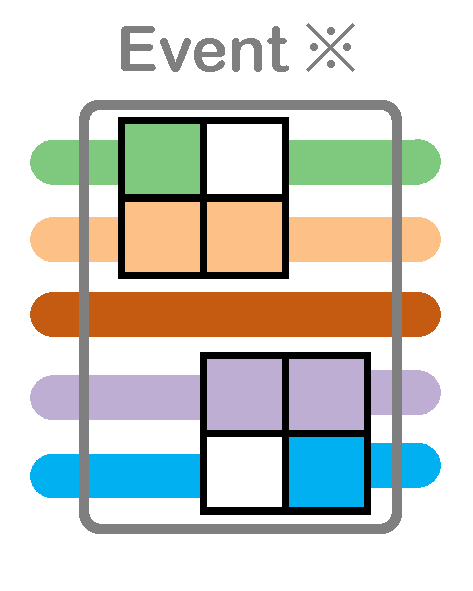
\includegraphics[width=\linewidth,height=3.5cm]{Fig/BadEG.pdf}}
		\vspace{-0.5em}
		\caption{BadEG}
		\label{fig:BadEG}
		\vspace{-1.5em}
	\end{minipage}
	\begin{minipage}[c]{0.69\linewidth}
		\vspace{0em}
		\centering
		\centerline{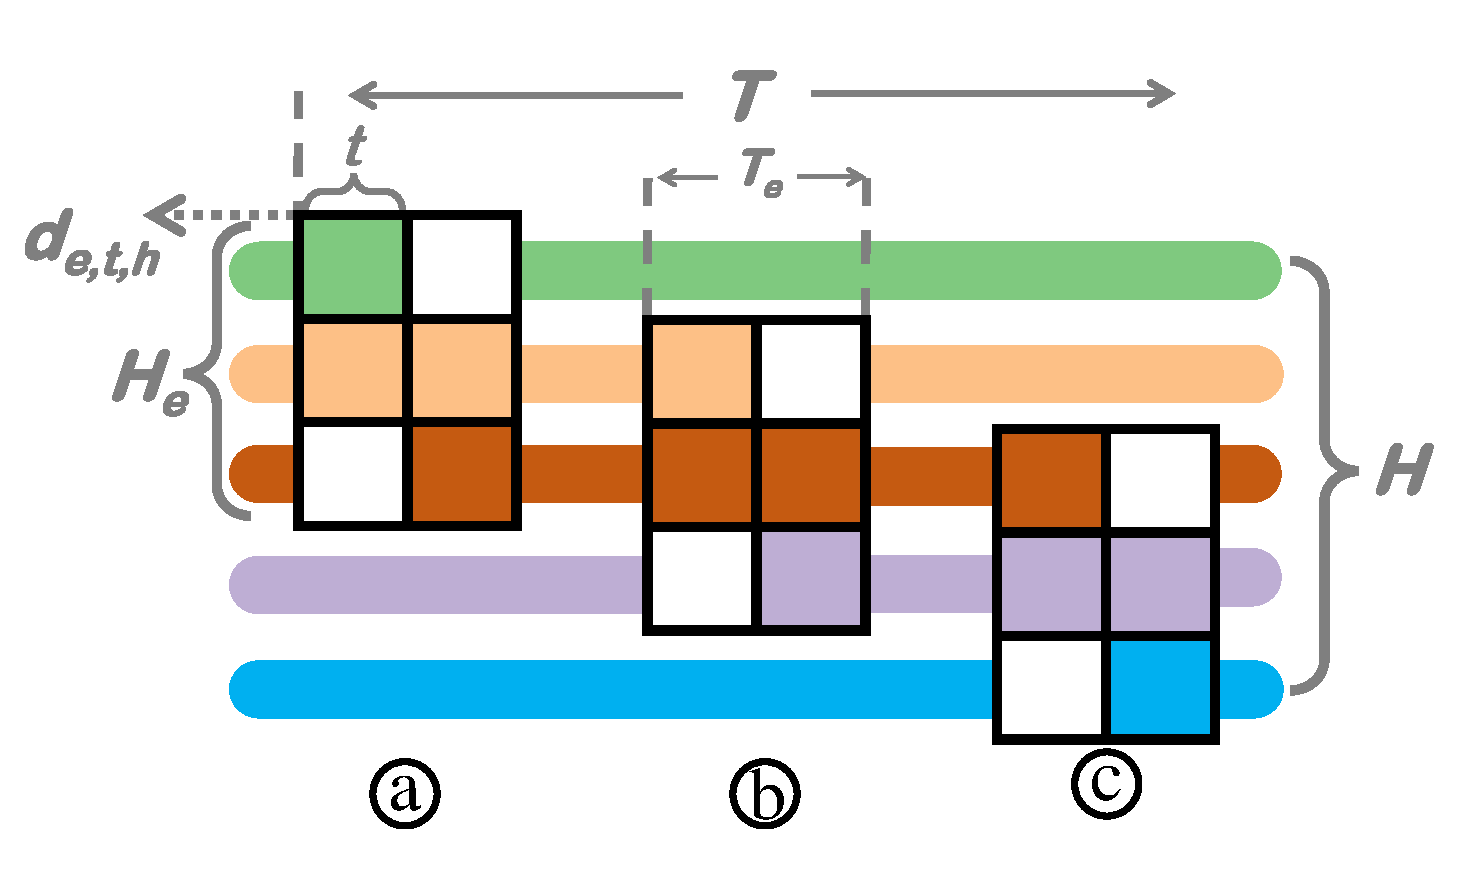
\includegraphics[width=\linewidth,height=4cm]{Fig/EG.pdf}}
		\vspace{-1em}
		\caption{EG}
		\label{fig:EG}
		\vspace{-1.5em}
	\end{minipage}
\end{figure}

%公式9
\begin{subequations}
	\begin{align}
	\sum_{h=0}^{H-H_e}d_{e,t,h}&=1, \quad\quad \forall e,t\;\; when\;\; B_{e,t} = 1\\
	\sum_{h=H-H_e+1}^{H-1}d_{e,t,h}&=0, \quad\quad \forall e,t\;\; when\;\; B_{e,t} = 1\\
	\sum_{i=0}^{H}\sum_{h_b=0}^{h-1}o_{i,t,h_b}C_{i,e}&=0, \quad\quad \forall e,t \;\;when\;\; d_{e,t,h}=1 \\
	\sum_{i=0}^{H}\sum_{h_e=h}^{h+H_e-1}o_{i,t,h_e}C_{i,e}&=H_e, \quad\quad \forall e,t \;\;when\;\; d_{e,t,h}=1
	\end{align}
\end{subequations}

%公式(9)详细描述了解决上述问题的算法。公式(9a)保证了当$h\in [0,\;H-H_e]$时,存在一个位置为窗口的起始点。公式(9b)保证了当$h\in [H-H_e+1,H-H-1]$时,不存在窗口的起始点。这样可以防止溢出。公式(9a)及(9b)两者组合保证了当$h\in[0, H-1]$时有且仅有一个点为窗口起始点。公式(9c)可以确保参与事件$e$的实体$i$不可能排在起始点$h$前。公式(9d)可以确保参与事件$e$的实体都在窗口内。
Eq.9 describes in detail the algorithm. Eq.(9a) ensures that when $h\in [0,\;H-H_e]$, there exists a location for the start of the window. Eq.(9b) ensures that when $h\in [H-H_e+1,H-H-1]$, there is no starting point for the window. This prevents overflow. Eq.(9a) and (9b) the combination of the two guarantees that when $h\in [0, H-1]$ there is and only one point for the start of the window. Eq.(9c) ensures that the entity $i$ involved in the event $e$ cannot be ranked in front of the starting point $h$. Eq.(9d) can ensure that the entities involved in the event $e$ are within the window.

%%算法1:窗口滑动
%\begin{algorithm} 
%	\caption{Aggregate the entities involved in event $e$} 
%	\label{alg1} 
%	\begin{algorithmic}
%		%输入:事件的数组,人员的数组,故事持续时间
%		\Require $Arr_{ev}$: an array of events; $Arr_{en}$: an array of entities; $T$: story duration; 
%		\For{$e$ in range(0,len($Arr_{ev}$))}
%			\State set $H_e$ = 0; $H = $len($Arr_{en}$)
%			\For{$i_e$ in range(0,$\;\;H$)}
%			 	%如果$Arr_{en}$中的实体$i$参与了$Arr_{en}$中的事件$e$,则H_e++
%			 	\State If entity $i_e$ in $Arr_{en}$ is involved in event $e$ in $Arr_{en}$, then $H_e++$;
%			\EndFor 
%			\For{$t$ in range($T$)}
%				%当时刻t发生了第x个事件	
%				\While{the event $e$ occurs at moment $t$}
%					\For{$h$ in range(0,$\;\;H-H_e+1$)}	
%						%确定窗口起点和终点的可能范围
%						\State $d(x,t,h)$, $h \in [0,\;\;H-H_e+1$);
%%						\Comment{Determine the starting point of the window}
%						\For{$i$ in range($0,\;\;H$)}
%							\For{$h_b$ in range($0,\;\;h-1$)}
%								%保证排在$h$前的实体都没有参与事件$e$
%								\State $o_{i,t,h_b}C_{i,e} = 0$;  					
%							\EndFor
%							\For{$h_e$ in range($h,\;\;h+H_e$)}
%								\State $o_{i,t,h_e}C_{i,e} = 1$;
%							\EndFor 
%						\EndFor
%					\EndFor
%				\EndWhile  
%			\EndFor
%		\EndFor
%	\end{algorithmic} 
%\end{algorithm}
